\documentclass[a4paper,12pt]{report}

\usepackage[utf8x]{inputenc}
\usepackage[T1]{fontenc}
\usepackage[french]{babel}
\usepackage{lmodern} % For changing the font
\usepackage{subcaption}

\usepackage{graphicx} % For including images
\usepackage{wrapfig} % For using images wrapped inside some text
\usepackage{hyperref} % For adding metadata information under \hypersetup
\usepackage{float} % The float package provides the H option to floating environments, which completely stops them from floating.

\PrerenderUnicode{é} % This is for fixing the issue or having index/header 'é' error

\hypersetup{
pdftitle={Conception et réalisation d'une plateforme d'échange de livre basée sur une application Android/iOS},
pdfsubject={Projet de Fin d’Etudes},
pdfauthor={Rahmouni Abdelhak},
pdfkeywords={Flutter, Android, iOS, Books}
}

%		Header		%		
\usepackage{fancyhdr}
\pagestyle{fancy}
\rhead{\thepage}
\lhead{\leftmark}

\usepackage{makeidx}
\makeindex
\usepackage[sort=use]{glossaries}

\makeglossaries

%from documentation
%\newacronym[⟨key-val list⟩]{⟨label ⟩}{⟨abbrv ⟩}{⟨long⟩}
%above is short version of this
% \newglossaryentry{⟨label ⟩}{type=\acronymtype,
% name={⟨abbrv ⟩},
% description={⟨long⟩},
% text={⟨abbrv ⟩},
% first={⟨long⟩ (⟨abbrv ⟩)},
% plural={⟨abbrv ⟩\glspluralsuffix},
% firstplural={⟨long⟩\glspluralsuffix\space (⟨abbrv ⟩\glspluralsuffix)},
% ⟨key-val list⟩}
 
 \newglossaryentry{GPS}
{
    name=GPS,
    description={Un Global Positioning System (GPS) est un système de géolocalisation par satellite}
}

\newglossaryentry{coordGPS}
{
    name=coordonnées,
    description={Les coordonnées géographiques permettent de localiser un lieu sur la Terre grâce à trois mesures : l'altitude, la longitude et la latitude. Les coordonnées géographiques sont notamment utilisées par les GPS}
}

\newglossaryentry{OpenStreetMap}
{
    name=OpenStreetMap,
    description={OpenStreetMap est un projet international fondé en 2004 dans le but de créer une carte libre du monde. Il collecte des données dans le monde entier sur les routes, voies ferrées, les rivières, les forêts, les bâtiments …}
}

\newglossaryentry{GoogleMaps}
{
    name=Google Maps,
    description={Google Maps est une application pour la manipulation de données géographiques, permettant entre autre, d'afficher les cartes du monde entier et de tracer des itinéraires entre deux points par exemple}
}

\newglossaryentry{plateforme}
{
    name=plateforme,
    description={une plateforme est un environnement permettant la gestion et/ou l'utilisation de logiciels et applications, elle peut désigner un système d'exploitation, un environnement d'exécution, un serveur...etc}
}

\newglossaryentry{SQL}
{
    name=SQL,
    description={SQL (Structured Query Language) est un langage informatique normalisé servant à exploiter des bases de données relationnelles}
}

\newglossaryentry{NoSQL}
{
    name=NoSQL,
    description={NoSQL désigne une famille SGBD qui s'écarte du paradigme classique des bases de données relationnelles}
}

\newglossaryentry{framework}
{
    name=framework,
    description={Un framework est une sorte d'infrastructure de développement, il désigne un ensemble cohérent de composants logiciels structurels qui sert à créer les fondations ainsi que les grandes lignes de tout ou d'une partie d'un logiciel ou application}
}

\newglossaryentry{librairie}
{
    name=bibliothèque,
    description={En informatique, une bibliothèque logicielle est une collection de fonctions, qui peuvent être déjà compilées et prêtes à être utilisées par des programmes}
}

\newglossaryentry{API}
{
    name=API,
    description={une API (Application Programming Interface) est un ensemble de règles et spécifications qu'un programme peut suivre pour accéder et faire usage des services et des ressources fournis par un autre programme particulier qui implémente cette API}
}

\newglossaryentry{JSONg}
{
    name=JSON,
    description={JavaScript Object Notation}
}
\newacronym{AOT}{AOT}{Ahead Of Time}

\newacronym{URL}{URL}{Uniform Resource Locator}

\newacronym{JSON}{JSON}{JavaScript Object Notation}

\begin{document}

\thispagestyle{empty}

\addcontentsline{toc}{chapter}{Remerciements}

\vspace*{5cm}

\begin{center}
\textbf{Remerciements}
\end{center}

Nous voudrions tout d’abord remercier notre encadrant, M. BENALLAL Mohammed Anis, pour avoir adapté a nous, au lieu de nous obliger à nous adapter à lui, d’avoir permis à notre créativité de s’épanouir tout en continuant de fournir les bons conseils qui nous ont été très utiles, et nous espérons avoir pu exprimer notre gratitude et notre reconnaissance à chaque rencontre.\medskip

Ensuite, nous soulignons l’impact considérable que nos collègues du club scientifique UDev ont eu sur nous en tant qu’étudiants, puis sur ce travail, merci.\medskip

Enfin, un grand salut à tous les rebelles, à ceux qui font les choses comme ils croient qu'elles devraient être faites.

\newpage

\thispagestyle{empty}

\vspace*{2cm}

\begin{center}
\textbf{Résumé}
\end{center}

Les livres ont toujours été le principal vecteur de connaissances tout au long de l'histoire, et l'une des pratiques les plus gratifiantes connues de l'humanité, heureusement, de nos jours encore, une grande partie de la population considère la lecture comme un mode de vie et le livre comme le meilleur compagnon qu'une personne puisse espérer avoir. Cependant, dans le monde actuel et plus particulièrement dans notre pays, l'Algérie, ce mode de vie est devenu de plus en plus difficile à maintenir, pour des raisons aussi diverses que le coût d'achat de certains livres, la difficulté d'en trouver d'autres et les difficultés rencontrées pour se connecter à d'autres lecteurs qui partagent les mêmes intérêts et amour pour la lecture.\medskip

Par conséquent, afin de résoudre ces problèmes, nous nous sommes tournés vers la technologie, en exploitant le pouvoir offert par les smartphones qui envahissent tous les poches et l’énorme popularité des réseaux sociaux, nous avons décidé de concevoir et de mettre en œuvre une application mobile.\medskip

Cette application mobile permet aux utilisateurs de définir un profil avec leur localisation géographique et de répertorier tous les livres qu'ils possèdent et qu’ils sont prêts à les prêtés, cédés, vendus ou échangés contre un autre livre avec un autre utilisateur. Cela leur permet également de parcourir le profil d'autres utilisateurs. Et leurs listes de livres dans l’espoir de trouver un livre qui les intéresse ou même un ami avec qui partager la passion de la lecture.\medskip

Nous avons pu ouvrir la voie en créant une conception détaillée et, plus tard, en développant les principales fonctionnalités en tenant compte des améliorations potentielles.

\tableofcontents
\listoffigures
%\listoftables --- until now I haven't used any tables
\printindex
\printglossary[type=main, title={Glossaire et acronymes}]

\newcommand\tab[1][0,4cm]{\hspace*{#1}}
\newcommand\longtab[1][1cm]{\hspace*{#1}}

\chapter{Généralités}
\section{Introduction au sujet}

\paragraph*{}
Ces dernières années, la communauté des lecteurs algériens a connu une croissance rapide et le taux de participation aux salons du livre est prometteur. Avec cette quantité de livres achetés, de nouveaux problèmes voient le jour, en plus des problèmes déjà existants tels que: les prix relativement élevés de certains livres, la rareté de certains autres et la tâche difficile que les lecteurs doivent endurer pour s'identifier avec d'autres membres qui partage les mêmes intérêts et la même zone géographique, se pose le problème de stockage de ces livres et du fait qu’ils peuvent être lu par un nouveau lecteur que de prendre de la place sur une étagère quelque part.


\paragraph*{}
Il existe des clubs de lecture et des réunions sociales où les gens échangent, vendent, donnent des livres et même rencontrent de nouvelles personnes, ce qui laisse penser qu'il existe un groupe de personnes qui:

\begin{list}{•}{}
	\item Ont des livres.
	\item Sont disposés à abandonner les livres déjà lus.
	\item Veulent économiser de l’argent tout en lisent de nouveau livres
\end{list}

\paragraph*{}
Comme nous venons de le dire, certaines solutions existent pour cette communauté et nous en explorerons certaines dans les sections suivantes tout en soulignant leurs lacunes et en expliquant comment une fenêtre d'opportunités est encore ouverte pour résoudre le problème dans ces différentes aspects.

\section{Solutions déjà existants}

\subsection{Non technologiques}

\paragraph*{}
L'analyse de cette question donnera lieu à deux concepts intéressants qui existent déjà et qui sont, dans une certaine mesure, fonctionnels:

\subparagraph{{\large 1. Événements d'échange de livres}\medskip\\}

Certains clubs de lecture et cafés organisent des événements où les participants sont invités à apporter les livres qu'ils souhaitent transmettre aux autres lecteurs et à en obtenir de nouveaux dans une atmosphère conviviale.

\subparagraph*{}
\begin{list}{•}{\textbf{Avantages}}
	\item Les participants peuvent vivre toute l'expérience humaine d'échanger un livre.
	\item Les participants découvrent de nouveaux livres par des personnes autres que des simple avis en ligne.
	\item Les participants établissent des liens significatifs avec leurs collègues lecteurs de livres.
\end{list}

\subparagraph*{}
\begin{list}{•}{\textbf{Inconvénients}}
	\item De tels événements durent au mieux 2 jours, ce qui fait que beaucoup de gens ratent l'occasion.
	\item En raison de la limitation géographique, de tels événements ne peuvent être accessibles que par quelques résidents proches de la région.
	\item coûteux en terme de temps investi.
\end{list}

\newpage

\subparagraph{{\large 2. Échanges informels de livres}\medskip\\}

Certains échanges de livres sont informels - une étagère ou une boîte est fournie où les livres peuvent être laissés ou ramassés. L'échange repose sur les utilisateurs qui sortent et prennent des livres et n'est généralement pas supervisé.\medskip

C'est une pratique courante dans les auberges de jeunesse où les voyageurs peuvent laisser un livre et emporter un livre différent avec eux. Certaines gares ferroviaires en Grande-Bretagne ont des échanges de livres informels et une a également été installée dans une cabine téléphonique à Kington Magna\cite{noauthor_book_2019}.

\subparagraph*{}
\begin{list}{•}{\textbf{Avantages}}
	\item Le processus est très rapide et pratiquement pas de temps perdu.
	\item Absence de limite de temps, ils peuvent être échangés à tout moment.
\end{list}

\subparagraph*{}
\begin{list}{•}{\textbf{Inconvénients}}
	\item Le besoin de donateurs au début du projet.
	\item L'absence d'un système de contrôle de qualité pour les livres mis contre les prises.
\end{list}

\begin{figure}[h]
	\begin{center}
		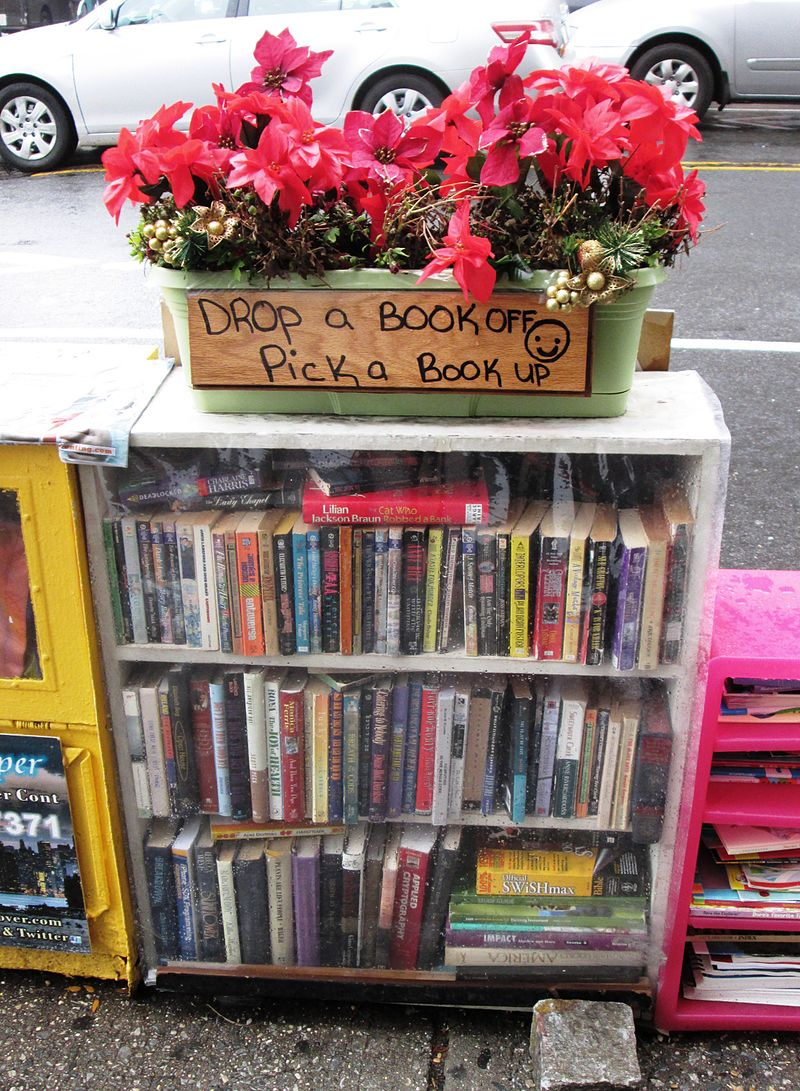
\includegraphics[width=5cm]{Images/chapter1/bookswapSpot.jpg}
		\caption{{\footnotesize Un "échange de livres de rue" à Washington Heights, New York\cite{noauthor_book_2019}}}
	\end{center}
\end{figure}

\newpage

\subsection{Technologiques}

\paragraph*{}
Il existe plusieurs sites Web et très peu d'applications populaires offrant le type de bonne expérience présente dans la manière traditionnelle, nous allons explorer certaines des plus populaires solutions existant aujourd’hui.\\

\subparagraph{{\large 1. BookMooch:}\medskip \\}

\begin{wrapfigure}[13]{r}{3.5cm}
	\raisebox{0pt}[\dimexpr\height+1.5\baselineskip\relax]{
\includegraphics[width=3.5cm]{Images/chapter1/bookMoochLogo.jpg}}
	\caption{{\footnotesize Logo de BookMooch}}
\end{wrapfigure}

Portant bien son nom, avec le fameux slogan \textit{​“Give books away, Get books you want”},BookMooch est une société de publication delivres en ligne par laquelle ses membres peuvent échanger des livres entre eux. Son fondateur,
John Buckman, a choisi ce nom pour l'entreprise en référence à l'acte de donner un livre sans attendre de le récupérer. Les utilisateurs, alors, sont considérés comme des BookMoochers et bénéficient à bien des égards de ce système commercial unique.

En bref, les utilisateurs «achètent» les livres des autres membres	en utilisant uniquement des points. Chaque membre peut accumuler des points en soumettant les titres des livres qu'il veut donner et en envoyant ses livres à d'autres utilisateurs. Avec suffisamment de points, ils peuvent alors commencer à recevoir les titres d'autres personnes, et le processus continue à partir de là. Le seul coût pour les membres est celui de l'envoi des livres qu'ils envoient à d'autres.\cite{noauthor_bookmooch_nodate}\\

\subparagraph*{}
\begin{list}{•}{\textbf{Avantages}}
	\item L'adhésion à cette entreprise est gratuite.
	\item Vous pouvez choisir parmi une grande variété de livres.
	\item Une liste de souhaits connectée à amazon où vous recevrez des notifications lorsque des livres sont disponibles.
\end{list}

\subparagraph*{}
\begin{list}{•}{\textbf{Inconvénients}}
	\item Pour recevoir, il faut donner.
	\item Dans une certaine mesure, la plate-forme peut être un terrain de jeu pour les fraudeurs.
	\item La plate-forme n'exploite pas l'emplacement des membres.
\end{list}

\subparagraph{{\large 2. Bookup:}\medskip \\}

\begin{wrapfigure}[8]{r}{2.5cm}
		\raisebox{0pt}[\dimexpr\height+2\baselineskip\relax]{
\includegraphics[width=2.5cm]{Images/chapter1/bookUpLogo.jpg}}
		\caption{{\footnotesize Logo de Bookup}}
\end{wrapfigure}

L'application Bookup est destinée aux lecteurs de livres imprimés qui souhaitent échanger leurs livres contre d'autres livres de leur région, gratuitement, et éventuellement se faire un nouvel ami partageant le même intérêt pour la lecture. Bookup fournit une fonctionnalité d’échange de livre en fonction de l’emplacement.\cite{noauthor_bookup_nodate-1}\\

\subparagraph*{}
\begin{list}{•}{\textbf{Avantages}}
	\item La plate-forme exploite l'emplacement des membres.
	\item Fonctionnalité de bibliothèque personnelle que vous pouvez personnaliser à votre guise.
	\item Liberté absolue pour les utilisateurs de discuter en temps réel et de trouver un moyen d'exécuter l'échange.
	\item Un mécanisme simple d'exploration aléatoire de livres proches.
\end{list}

\subparagraph*{}
\begin{list}{•}{\textbf{Inconvénients}}
	\item L'application est disponible uniquement sur les appareils marchent avec iOS.
	\item Une expérience utilisateur moyenne.
	\item Un manque évident d'informations sur les livres et les utilisateurs.
\end{list}

\begin{figure}[h]
	\begin{center}
		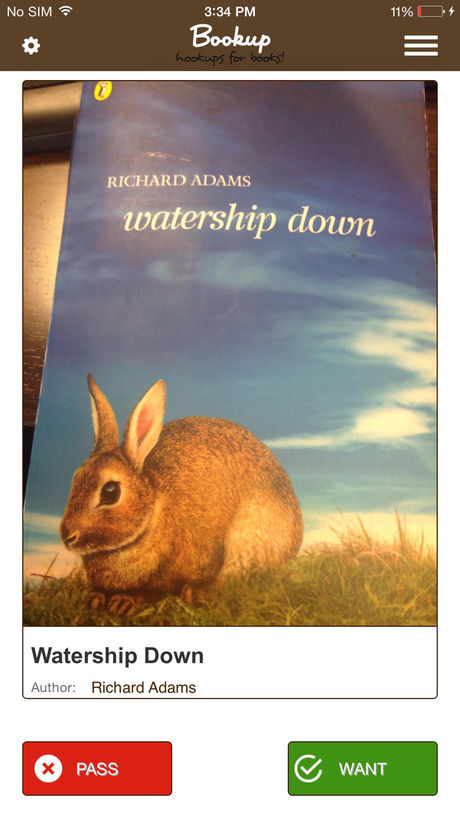
\includegraphics[width=3cm]{Images/chapter1/bookUpScreenshot.jpg}
		\caption{\footnotesize {Le mecanisme de suggestion et decouverte offert par Book Up ou l'utilisateur parcours une pile de cartes des livres près de son zone géographique on choisissent “passer” ou “vouloir”}}
	\end{center}
\end{figure}
\newpage

\subparagraph{{\large 3. Bookabikia\medskip \\}}

%raisedbox is for adding margin to wrapfigure
\begin{wrapfigure}[9]{r}{4cm}
	\raisebox{0pt}[\dimexpr\height+2.5\baselineskip\relax]{
\includegraphics[width=4cm]{Images/chapter1/bookabikiaLogo.png}}
	\caption{{\footnotesize Logo de Bookabikia}}
\end{wrapfigure}

Bookabikia est une plate-forme et un service fabriqués en Égypte qui permettent aux gens d'échanger des livres. L'équipe derrière le projet a fait un excellent travail en résolvant non seulement les problèmes évidents auxquels la communauté des lecteurs est confrontée, mais également en l'exploitant avec brio. Sur le site Bookabkia, vous ferez une demande de don pour le site avec vos livres. L’équipe de livraison viendra à vous pour prendre les livres dans les jours à venir et 24 heures après avoir reçu les livres, vous obtiendrez un crédit qui se présente sous forme de points, avec ce crédit, vous pourrez acheter plusieurs livres en même temps sans avoir besoin d’intérêt personnel pour vos livres.\cite{noauthor_bookabikia_nodate}

\subparagraph*{}
\begin{list}{•}{\textbf{Avantages}}
	\item Les utilisateurs ne sont pas obligés de passer des offres d'échange avec d'autres utilisateurs.
	\item La fonction de crédit donne beaucoup de liberté de choix aux gens.
	\item Tous les livres sont expédiés au domicile de l'utilisateur.
\end{list}

\subparagraph*{}
\begin{list}{•}{\textbf{Inconvénients}}
	\item La plate-forme ne permet pas les interactions peer-to-peer entre les membres de la communauté.
	\item Le service n'est pas totalement gratuit.
	\item L'expérience utilisateur n'est pas personnalisable.
\end{list}

\begin{figure}[h]
	\begin{center}
		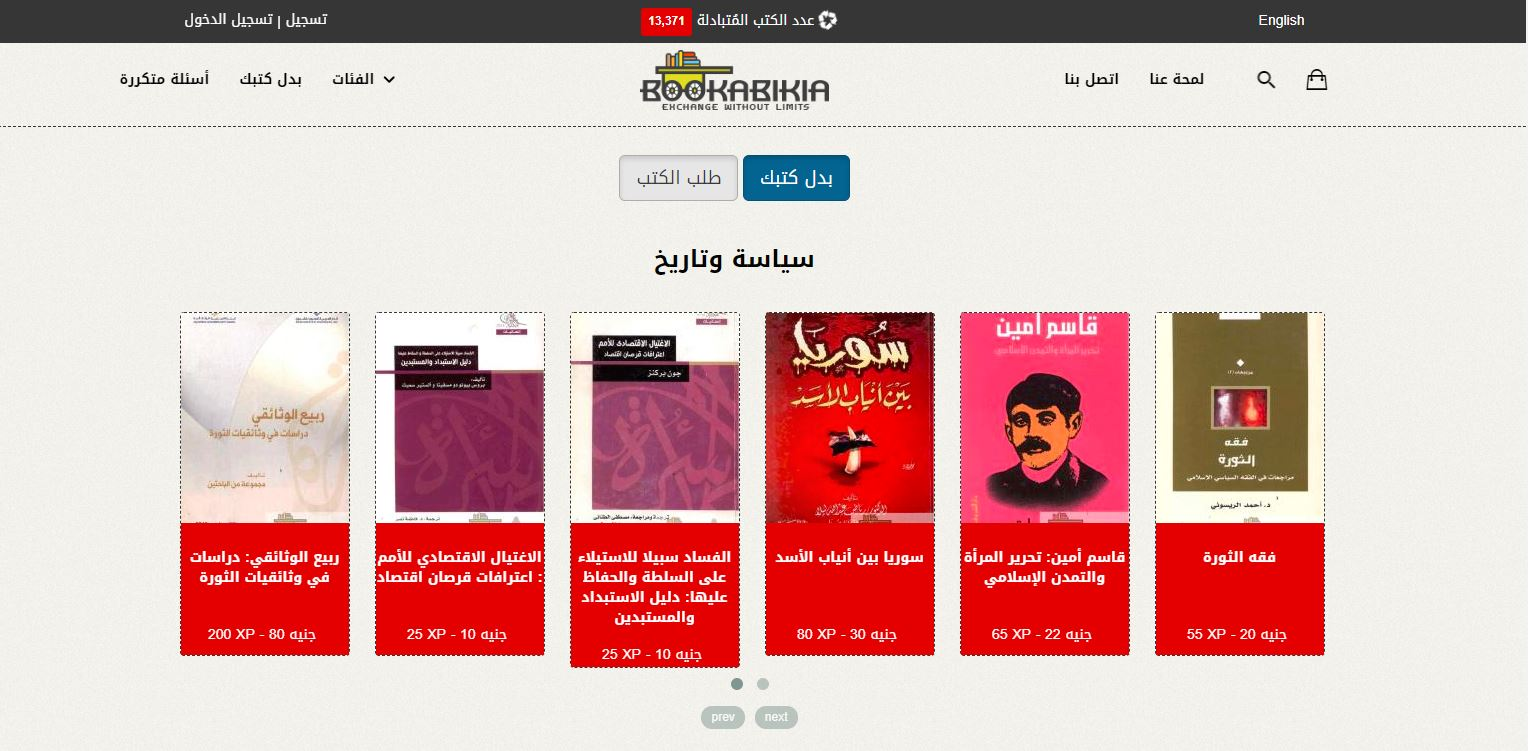
\includegraphics[width=9cm]{Images/chapter1/bookabikiaScreenshot.jpg}
		\caption{{\footnotesize Page d'acceuil de Bookabikia}}
	\end{center}
\end{figure}

\newpage
\section{Solution proposé}
\paragraph*{}
Aussi merveilleux que les solutions existantes sont, nous pensons pouvoir encore offrir une meilleure solution et une meilleure expérience, en exploitant deux aspects de la pratique de l'échange de livres:

\begin{list}{•}{}
	\item La sociabilité humaine et la capacité à s'identifier aux autres et à créer de petites communautés et des relations durables et significatives.
	\item Une interface utilisateur magnifique et une expérience utilisateur personnalisable qui permettent une totale liberté d'interaction avec d'autres utilisateurs.
\end{list}

La solution consiste en une application mobile fonctionnant à la fois sur Android et sur iOS (97,43\% des appareils du monde \cite{noauthor_mobile_nodate}), où les utilisateurs enregistrés peuvent:

\begin{list}{•}{}
	\item Créez un profil et répertoriez tous les livres qu’ils possèdent et sont disposés à échanger, prêter, vendre ou même faire un don à un autre utilisateur de leur choix. Le tout dans une interface utilisateur magnifiquement structuré.
	\item Recherchez les livres qu'ils souhaitent acquérir en utilisant des mécanismes de recherche avancés qui permettent d'obtenir les résultats les plus homogènes, les plus fonctionnels et les plus pratiques.
	\item Explorez les utilisateurs à proximité (propriétaires de livres) a l'aide de la map, parcourez leurs bibliothèques d'un simple balayage et d'un clic.
	\item Envoyez et recevez des messages en temps réel avec le service de messagerie, sans aucune limitation.
\end{list}

Enfin, l’application portera le nom «Bindex», qui est une forme abrégée d’index de livre qui résume le travail que l’application accomplit en indexant toutes les bibliothèques personnelles et en les mettant au bout du doigt d’un utilisateur donné.

\begin{figure}[h]
	\begin{center}
		\raisebox{0pt}[\dimexpr\height+2\baselineskip\relax]{
\includegraphics[width=6.5cm]{Images/chapter1/bindexLogo.png}}
		\caption{{\footnotesize Logo de Bindex}}
	\end{center}
\end{figure}

\section{Plan du rapport}
\paragraph*{}
Après avoir passé en revue les généralités et l’introduction, nous plongerons dans la manière dont ce projet prospère va prendre vie:
\paragraph*{}
Dans le deuxième chapitre, nous aborderons les technologies et les solutions les plus appropriées pour la réalisation de l’application mobile, en mentionnant également certains services de base utilisés, et dans le chapitre suivant, nous aborderons les processus qui ont été pris en compte pour la création. de l’application, de la conception initiale et brouillon au prototypage, tout en soulignant les outils utilisés, ainsi que les mécanismes de co-travail et les outils qui ont permis de faire de l’ensemble du projet une expérience fluide.
\paragraph*{}
Après cela, nous plongerons encore plus profondément dans une démonstration où nous présenterons toutes les fonctionnalités qui ont été développées et comment nous prévoyons de nous développer à l’avenir.




\chapter{Les technologies utilisées}

\section{Un bref historique du développement d'applications mobiles}
Le développement d'applications mobiles est l'acte ou le processus par lequel une application est développée pour les appareils mobiles. Ces applications peuvent être préinstallées sur les téléphones au cours de la fabrication ou accessibles via un navigateur Web \cite{noauthor_mobile_2019}. Toutefois, au cours de la dernière décennie \cite{leler_whats_2017}, des développeurs tiers ont été capables de créer des applications mobiles. Cependant, en raison de la concurrence intense dans les logiciels mobiles et des modifications apportées à chacune des plateformes, ces développeurs doivent prendre en compte un large éventail de tailles d'écran, de spécifications matérielles et de configurations.

Le développement d'applications mobiles est un domaine d'activité relativement récent. il n’est donc pas surprenant que les outils évoluent encore.
\newpage

\subsection{Les kits de développement de plate-forme (Platform SDKs)}
Le SDK Apple iOS est sorti en 2008 et le SDK Google Android en 2009. Ces deux SDK étaient basés sur des langages différents: Objective-C et Java, respectivement.
Votre application communique avec la plateforme pour créer des widgets ou accéder à des services tels que la caméra. Les widgets sont rendus dans un canevas d’écran et les événements sont renvoyés aux widgets. C'est une architecture simple, mais vous devez créer des applications séparées pour chaque plate-forme car les widgets sont différents, sans parler des langues natives\cite{leler_whats_2017}.

\begin{figure}[h]
	\begin{center}
		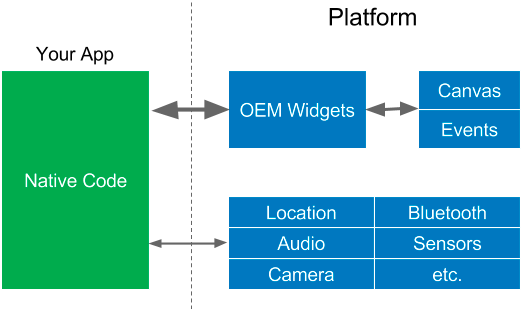
\includegraphics[width=10cm]{Images/chapter2/platform_sdk.png}
		\caption{{\footnotesize Architecture du développement mobile a l'aide des SDK\cite{leler_whats_2017}}}
	\end{center}
\end{figure}

\subsection{Vues Web (WebViews)}
Les premiers frameworks multi-plateformes étaient basés sur JavaScript et WebViews. Les exemples incluent une famille de frameworks liés: PhoneGap, Apache Cordova, Ionic, etc. Avant de publier leur SDK iOS, Apple avait encouragé les développeurs tiers à créer des applications Web pour iPhone. Il était donc évident de créer des applications multiplates-formes à l'aide de technologies Web.

\begin{figure}[h]
	\begin{center}
		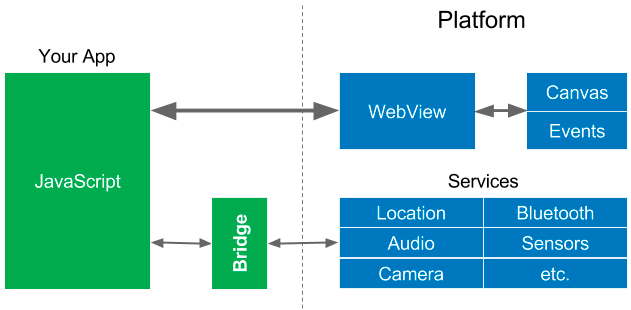
\includegraphics[width=11cm]{Images/chapter2/webview.png}
		\caption{{\footnotesize Architecture du développement mobile a l'aide des WebViews\cite{leler_whats_2017}}}
	\end{center}
\end{figure}

Votre application crée du HTML et l'affiche dans une vue Web sur la plateforme. Notez qu'il est difficile pour des langages tels que JavaScript de parler directement au code natif (comme les services), de sorte qu'ils passent par un «pont» qui fait que le contexte bascule entre le domaine JavaScript et le domaine natif. Comme les services de plate-forme ne sont généralement pas appelés très souvent, cela n’a pas causé trop de problèmes de performances\cite{leler_whats_2017}.

\subsection{Vues réactives (Reactive Views)}
Les infrastructures Web réactives telles que ReactJS (et d'autres) sont devenues populaires, principalement parce qu'elles simplifient la création de vues Web grâce à l'utilisation de modèles de programmation empruntés à la programmation réactive. En 2015, React Native a été créé pour apporter les nombreux avantages des vues réactives aux applications mobiles.\\

\begin{figure}[h]
	\begin{center}
		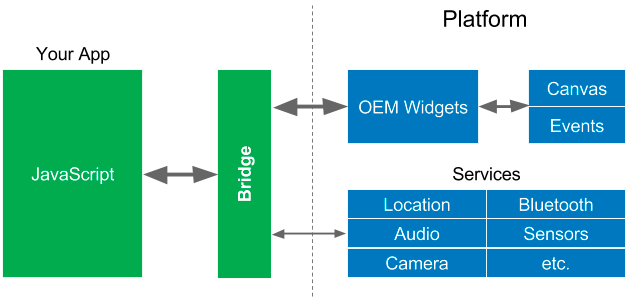
\includegraphics[width=11cm]{Images/chapter2/reactive_views.png}
		\caption{{\footnotesize Architecture du développement mobile a l'aide des Reactive Views\cite{leler_whats_2017}}}
	\end{center}
\end{figure}

\begin{wrapfigure}[8]{r}{2cm}
	
\includegraphics[width=2cm]{Images/chapter2/react_native_logo.png}
	\caption{{\footnotesize Logo de React Native}}
\end{wrapfigure}

React Native est très populaire (et mérite de l'être), mais comme le domaine JavaScript accède aux widgets de la plate-forme dans le domaine natif, il doit également passer par le pont. Les widgets sont généralement utilisés assez fréquemment (jusqu'à 60 fois par seconde lors d'animations, de transitions ou lorsque l'utilisateur balaie quelque chose sur l'écran avec son doigt), ce qui peut entraîner des problèmes de performances.

\section{Flutter}

\subsection{Qu'est-ce que Flutter?}

\begin{wrapfigure}[8]{r}{2cm}
	
\includegraphics[width=2cm]{Images/chapter2/flutter_logo.png}
	\caption{{\footnotesize Logo de Flutter}}
\end{wrapfigure}

Flutter est un SDK pour applications mobiles permettant de créer des applications hautes performances et haute fidélité pour iOS et Android à partir d'une seule base de code\cite{noauthor_technical_nodate}.\medskip

L'objectif est de permettre aux développeurs de proposer des applications hautes performances qui se sentent naturelles sur différentes plates-formes. Nous adoptons des différences dans les comportements de défilement, la typographie, les icônes, etc.\bigskip

\begin{figure}[h]
	\begin{center}
		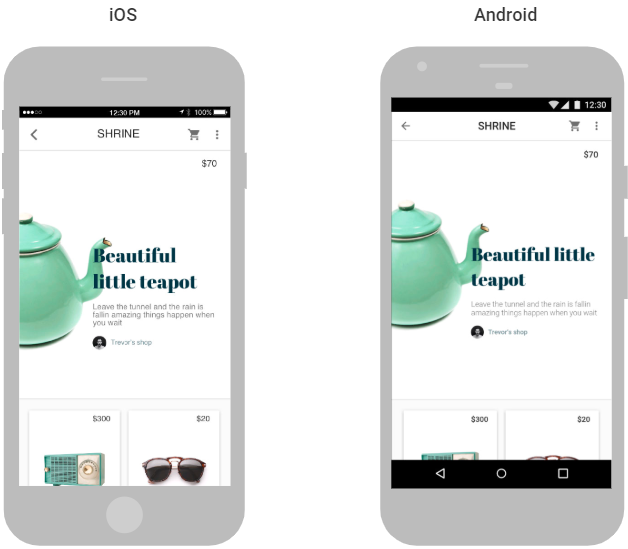
\includegraphics[width=9cm]{Images/chapter2/flutter_android_ios.png}
		\caption{{\footnotesize Ceci est une application de démonstration nommée Shrine\cite{noauthor_technical_nodate}}}
	\end{center}
\end{figure}

Comme React Native, Flutter fournit également des vues de style réactif. Flutter adopte une approche différente pour éviter les problèmes de performances causés par la nécessité d'un pont JavaScript en utilisant un langage de programmation compilé, à savoir Dart. Dart est compilé «à l'avance» \acrshort{AOT} en code natif pour plusieurs plates-formes. Cela permet à Flutter de communiquer avec la plate-forme sans passer par un pont JavaScript qui effectue un changement de contexte. La compilation en code natif améliore également les temps de démarrage des applications.\medskip

Flutter a une nouvelle architecture qui inclut des widgets qui ont l’air agréable, qui sont rapides, personnalisables et extensibles. il n'utilise pas les widgets de plate-forme (ou DOM WebViews), il fournit ses propres widgets.

\begin{figure}[h]
	\begin{center}
		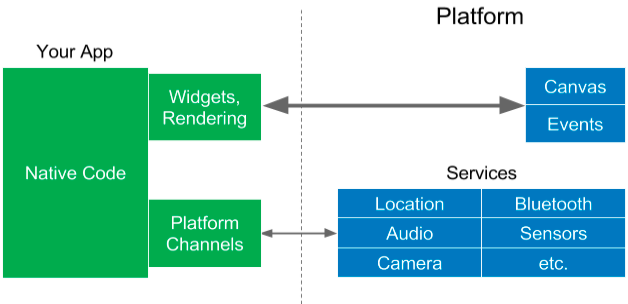
\includegraphics[width=11cm]{Images/chapter2/flutter.png}
		\caption{{\footnotesize Architecture du développement mobile a l'aide de Flutter\cite{leler_whats_2017}}}
	\end{center}
\end{figure}

Flutter soulève les widgets et le moteur de rendu de la plateforme dans l'application, ce qui leur permet d'être personnalisables et extensibles. Tout ce que Flutter a besoin de la plate-forme est un canevas dans lequel les widgets doivent être rendus afin qu’ils puissent apparaître sur l’écran du périphérique, ainsi que l’accès aux événements (touches, minuteries, etc.) et aux services (localisation, caméra, etc.).\medskip

Il existe toujours une interface entre le programme Dart (en vert) et le code de la plate-forme native (en bleu, pour iOS ou Android) qui effectue l’encodage et le décodage des données, mais cela peut être beaucoup plus rapide qu’un pont JavaScript.

\subsection{Principes de base}
Flutter comprend un \gls{framework} de style réact moderne, un moteur de rendu 2D, des widgets prêts à l'emploi et des outils de développement. Ces composants fonctionnent ensemble pour vous aider à concevoir, créer, tester et déboguer des applications. Tout est organisé autour de quelques principes fondamentaux.
\subsubsection{{\large 1 - Tout est un widget}}
Les widgets sont les éléments de base de l’interface utilisateur d’une application Flutter. Chaque widget est une déclaration immuable d'une partie de l'interface utilisateur. Contrairement aux autres frameworks qui séparent les vues, les contrôleurs de vue, les présentations et d'autres propriétés, Flutter possède un modèle objet cohérent et unifié: le widget.
Un widget peut définir:

\begin{list}{•}{}
	\item un élément structurel (comme un bouton ou un menu).
	\item un élément stylistique (comme une police ou un jeu de couleurs).
	\item un aspect de la mise en page (comme le rembourrage).
	\item etc…
\end{list}

Les widgets forment une hiérarchie basée sur la composition. Chaque widget niche à l'intérieur et hérite des propriétés de son parent. Il n'y a pas d'objet «application» séparé. Au lieu de cela, le widget racine joue ce rôle.
Vous pouvez répondre à des événements, comme une interaction utilisateur, en indiquant au cadre de remplacer un widget de la hiérarchie par un autre. La structure compare ensuite les nouveaux et les anciens widgets et met efficacement à jour l'interface utilisateur.\bigskip

\longtab \textbf{Composition> héritage\medskip}

Les widgets sont souvent eux-mêmes composés de nombreux petits widgets à usage unique qui se combinent pour produire des effets puissants. Par exemple, Container, un widget couramment utilisé, est composé de plusieurs widgets responsables de la mise en page, de la peinture, du positionnement et du dimensionnement. Plus précisément, Container est composé des widgets LimitedBox, ConstrainedBox, Align, Padding, DecoratedBox et Transform. Plutôt que de sous-classer Container pour produire un effet personnalisé, vous pouvez composer ces widgets simples, ainsi que d'autres, de manière innovante.\medskip

\begin{figure}[h]
	\begin{center}
		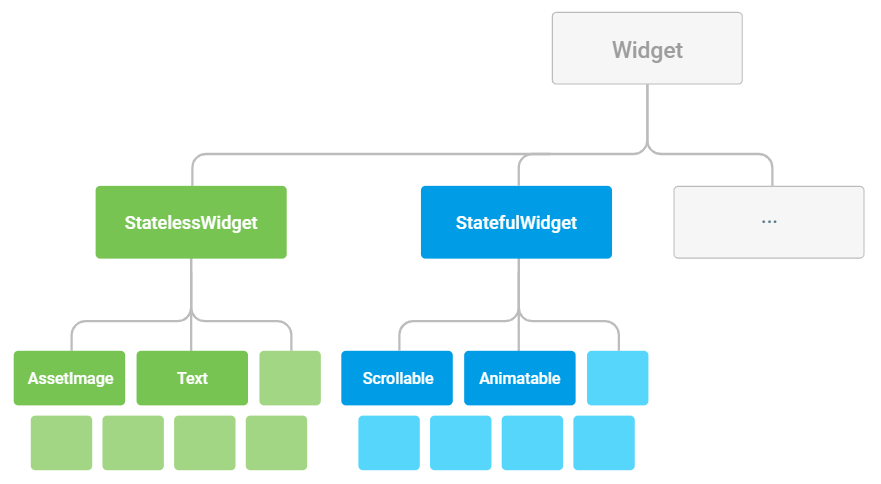
\includegraphics[width=13cm]{Images/chapter2/hierarchy_widgets.png}
		\caption{{\footnotesize Exemple d'une hierarchy des widgets\cite{noauthor_technical_nodate}}}
	\end{center}
\end{figure}

La hiérarchie des classes est peu profonde et large afin de maximiser le nombre possible de combinaisons.\medskip

Vous pouvez également contrôler la mise en page d'un widget en le composant avec d'autres widgets. Par exemple, pour centrer un widget, vous l'enroulez dans un widget Centre. Il existe des widgets pour le remplissage, l'alignement, les lignes, les colonnes et les grilles. Ces widgets de présentation ne possèdent pas de représentation visuelle. Au lieu de cela, leur seul objectif est de contrôler un aspect de la présentation d’un autre widget. Pour comprendre pourquoi un widget est rendu d’une certaine manière, il est souvent utile d’inspecter les widgets voisins.\bigskip

\longtab \textbf{Couches de framework Flutter\medskip}

Le framework Flutter est organisé en une série de couches, chaque couche s'appuyant sur la couche précédente.\medskip

\begin{figure}[h]
	\begin{center}
		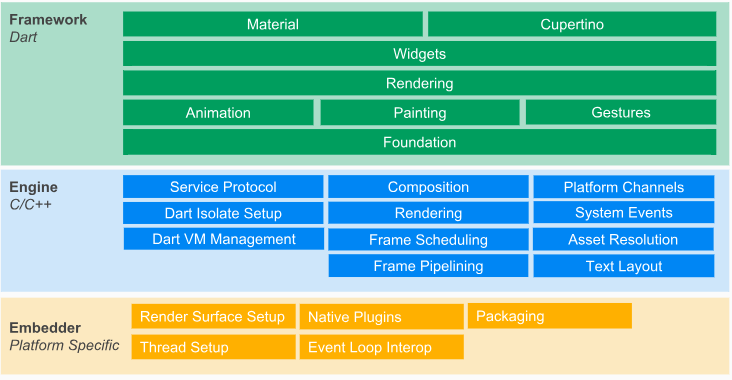
\includegraphics[width=13cm]{Images/chapter2/flutter_architecture.png}
		\caption{{\footnotesize L'architecture de flutter\cite{noauthor_technical_nodate}}}
	\end{center}
\end{figure}

Les couches supérieures du cadre sont utilisées plus fréquemment que les couches inférieures.\medskip

Le but de cette conception est de vous aider à faire plus avec moins de code. Par exemple, le calque Matérial est construit en composant les widgets de base à partir du calque Widgets, et le calque Widgets lui-même est construit en orchestrant des objets de niveau inférieur à partir du calque de rendu.
Les couches offrent de nombreuses options pour créer des applications.

Choisissez une approche personnalisée pour libérer toute la puissance d'expression du framework, ou utilisez des blocs de construction de la couche de widgets, ou combinez-les. Vous pouvez composer les widgets prêts à l'emploi fournis par Flutter ou créer vos propres widgets personnalisés à l'aide des mêmes outils et techniques que ceux utilisés par l'équipe Flutter pour créer le framework.

\subsubsection{{\large 2 - La construction de widgets}}
Vous définissez les caractéristiques uniques d'un widget en implémentant une fonction de génération qui renvoie une arborescence (ou une hiérarchie) de widgets. Cet arbre représente la partie de l’interface utilisateur du widget de manière plus concrète. Par exemple, un widget de barre d'outils peut avoir une fonction de génération qui renvoie une disposition horizontale de texte et de divers boutons. Le framework demande ensuite de manière récursive à chacun de ces widgets de construire jusqu'à ce que le processus se transforme en widgets entièrement concrets, que le framework assemble ensuite en un arbre.\medskip

La fonction de génération d’un widget doit être exempte d’effets secondaires. À chaque fois qu'il est invité à construire, le widget doit renvoyer une nouvelle arborescence de widgets, quel que soit ce que le widget a précédemment renvoyé. Le cadre fait beaucoup pour comparer la version précédente à la version actuelle et pour déterminer les modifications à apporter à l'interface utilisateur.\medskip

Cette comparaison automatisée est assez efficace, permettant des applications interactives hautes performances. Et la conception de la fonction de construction simplifie votre code en vous concentrant sur la déclaration d'un widget, plutôt que sur la complexité de la mise à jour de l'interface utilisateur d'un état à un autre.

\subsubsection{{\large 3 - Gestion de l'interaction utilisateur}}
Si les caractéristiques uniques d'un widget doivent être modifiées en fonction de l'interaction de l'utilisateur ou d'autres facteurs, ce widget est avec état. Par exemple, si un widget a un compteur qui s'incrémente chaque fois que l'utilisateur appuie sur un bouton, la valeur du compteur correspond à l'état de ce widget.\medskip
 
Lorsque cette valeur change, le widget doit être reconstruit pour mettre à jour l'interface utilisateur.\medskip

\begin{figure}[h]
	\begin{center}
		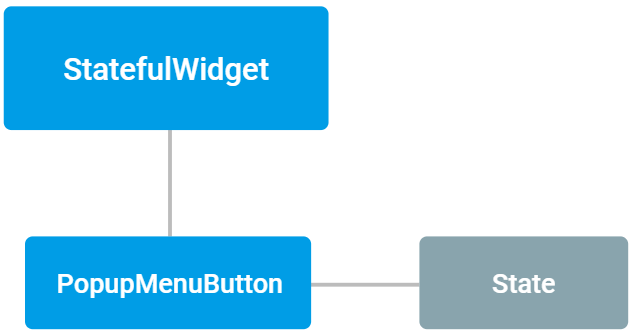
\includegraphics[width=10cm]{Images/chapter2/user_interaction_graph.png}
		\caption{{\footnotesize Modele d'une Widget Stateful\cite{noauthor_technical_nodate}}}
	\end{center}
\end{figure}

Ces widgets sous-classent StatefulWidget (plutôt que StatelessWidget) et stockent leur état mutable dans une sous-classe d’État.\medskip

Chaque fois que vous modifiez un objet State (par exemple, incrémentez le compteur), vous devez appeler setState() pour indiquer au framework de mettre à jour l'interface utilisateur en appelant à nouveau la méthode de compilation de State.\medskip

Avoir des objets state et widget séparés permet à d'autres widgets de traiter les widgets sans état et avec état de la même manière, sans craindre de perdre un état. Plutôt que de devoir conserver un enfant pour préserver son état, le parent est libre de créer une nouvelle instance de l'enfant sans perdre son état persistant. La structure fait tout le travail de recherche et de réutilisation des objets d'état existants, le cas échéant.


\subsection{Pourquoi utiliser Flutter?}
Comme nous l'avons mentionné précédemment, il existe de nombreuses options pour développer une application mobile, qu'il s'agisse de SDK natifs ou de frameworks multiplates-formes (Xamarin, ReactNative, Ionic, PhoneGap). Pour ce projet particulier, le framework Flutter a été choisi pour plusieurs points, dont les principaux sont:


\subsubsection{1. Multiplate-forme (cross-platform)}
Un produit ou système informatique multiplate-forme est un produit ou système pouvant fonctionner sur plusieurs types de plates-formes ou d'environnements d'exploitation.

Différents types de systèmes multiplates-formes incluent des systèmes matériels et logiciels, ainsi que des systèmes qui impliquent des versions séparées pour chaque plate-forme, ainsi que d'autres systèmes plus vastes conçus pour fonctionner de la même manière sur plusieurs plates-formes.
La plateforme croisée est également connue en tant que plate-forme indépendante\cite{noauthor_what_nodate}

Flutter offre la possibilité de créer une application compilée pour fonctionner à la fois sur Android et iOS à partir de la même base de code. Tout en maintenant l'expérience utilisateur appropriée sur chaque plate-forme.


\subsubsection{2. Productivité}
Flutter offre une augmentation de la productivité que provient du «rechargement à chaud» de Flutter («Stateful Hot Reload» et «Hot Restart». Ensemble, ils permettent aux développeurs de voir les modifications apportées à l'état d'une application en moins d'une seconde; structure de l'application en moins de dix.

Il n’est pas nécessaire d’exécuter une autre version de Gradle. Vous voyez vos modifications dès que vous enregistrez. Pour les développeurs, cela est souvent très facile à maîtriser - il n’ya que peu ou pas de courbe d’apprentissage liée à l’utilisation du «rechargement à chaud» car, par défaut, cela se produit chaque fois que vous enregistrez. Cependant, les avantages sont essentiels. Le temps de développement est souvent réduit de 30\% à 40\%, car les délais de reconstruction de Gradle qui ralentissent le développement des développeurs Android prennent généralement plus de temps à chaque modification appliquée.

\subsubsection{3. Intégration directe avec Firebase}
Firebase fournit un support prêt à l'emploi pour un ensemble de services tels que le stockage en nuage, les fonctions de nuage, les bases de données en temps réel, l'hébergement, l'authentification et bien plus encore. Votre infrastructure est instantanément sans serveur, redondante et évolutive. Cela signifie que vous n’avez pas à passer beaucoup de temps et de ressources à construire le backend. Il est également simple de le combiner avec un outil permettant d’automatiser votre processus de développement et de publication, tel que Fastlane; faciliter la livraison continue. Par conséquent, vous n'avez pas besoin de support DevOps dédié dans votre équipe.

\subsubsection{4. Performance}
L'application est compilée à l'avance en code ARM natif, pas au moment de l'exécution, comme dans React Native. Cela donne de meilleures performances car il n’ya pas de pont JS au milieu pour analyser et exécuter le code.

\subsubsection{5. L'utilisation de Dart}

\begin{wrapfigure}[7]{r}{5cm}
	
\includegraphics[width=5cm]{Images/chapter2/dart_logo.png}
	\caption{{\footnotesize Logo de Dart}}
\end{wrapfigure}

Dart est un langage de programmation polyvalent développé à l'origine par Google et ensuite approuvé en tant que norme par Ecma (ECMA-408). Il est utilisé pour créer des applications Web, serveur, bureau et mobiles.

Dart est un langage basé sur les objets, orienté objet, défini par la classe et utilisant une syntaxe de style C qui transcompile éventuellement en JavaScript. Il prend en charge les interfaces, mixins, classes abstraites, génériques réifiés, typage statique et un système de type sonore.\cite{noauthor_dart_2019}\medskip

Voici une liste rapide des fonctionnalités de Dart qui, ensemble, le rendent indispensable pour Flutter:

\begin{list}{•}{}
\item Dart est \acrshort{AOT} compilé en un code natif rapide et prévisible, qui permet à presque tout de Flutter d'être écrit en Dart. Cela rend non seulement Flutter rapide, mais pratiquement tout (y compris tous les widgets) peut être personnalisé.
\item Dart peut également être compilé \acrshort{JIT} (Just In Time) pour des cycles de développement exceptionnellement rapides et un flux de travail révolutionnaire (y compris le populaire rechargement à chaud avec état sous la seconde de Flutter).
\item Dart facilite la création d'animations lisses et de transitions exécutées à 60 images par seconde. Dart peut faire l’allocation d’objets et la collecte de place sans verrous. Et comme JavaScript, Dart évite la planification préemptive et la mémoire partagée (et donc les verrous). Les applications Flutter étant compilées en code natif, elles ne nécessitent pas de pont lent entre les domaines (par exemple, JavaScript vers natif). Ils démarrent aussi beaucoup plus vite.
\item Dart permet à Flutter d’éviter le recours à un langage de présentation déclaratif distinct, tel que \acrshort{JSX} ou \acrshort{XML}, ou à des générateurs d’interface visuelle distincts, car la présentation déclarative et programmatique de Dart est facile à lire et à visualiser. Et avec toute la mise en page dans une langue et à un endroit, il est facile pour Flutter de fournir des outils avancés qui facilitent la mise en page.
\item Les développeurs ont découvert que Dart est particulièrement facile à apprendre car il comporte des fonctionnalités bien connues des utilisateurs de langages statiques et dynamiques.
\end{list}

Toutes ces fonctionnalités ne sont pas propres à Dart, mais leur combinaison constitue un atout qui confère à Dart une puissance unique pour la mise en œuvre de Flutter. Tant pis, il est difficile d’imaginer que Flutter soit aussi puissant qu’il est sans Dart.\cite{leler_why_2018}


\section{Firebase}

\section{Google Maps}

\section{Google Books}
\chapter{Conception et implémentation de l’application}

\section{Conception}

\subsection{Introduction}
Tout comme la construction d’une maison nécessite des plans à différents niveaux (vision extérieure, plan des différents étages, plans techniques…), la réalisation d’une application informatique ou d’un ensemble d’applications est basée sur plusieurs diagrammes. Ces diagrammes doivent unifier la vision de l’équipe de développement et l’orienter vers la création d’une solution bien alignée sur les exigences du problème, et permettre également à l’équipe de proposer à ses clients une expérience utilisateur cohérente tout au long de l’application. 

Pour atteindre l'objectif de communiquer une vision ou un système difficile à expliquer par des mots, différents langages de modélisation ont été créés, tels que SysML, BON et le langage \acrshort{UML} le plus connu et le plus utilisé, ainsi que des méthodes anciennes et récentes, telles que le wireframing.

La pratique des conceptions logicielles n’est pas une pratique rigide dans laquelle plusieurs étapes clés sont toujours présentes dans un ordre particulier, par exemple : Le langage UML ne préconise aucune démarche, ce n’est donc pas une méthode. Chacun est libre d’utiliser les types de diagramme qu’il souhaite, dans l’ordre qu’il veut. Il suffit que les diagrammes réalisés soient cohérents entre eux, avant de passer à la réalisation du logiciel.

\subsection{Diagrammes de base}
\subsubsection{Diagrammes de séquence}

\begin{figure}[h]
	\begin{center}
		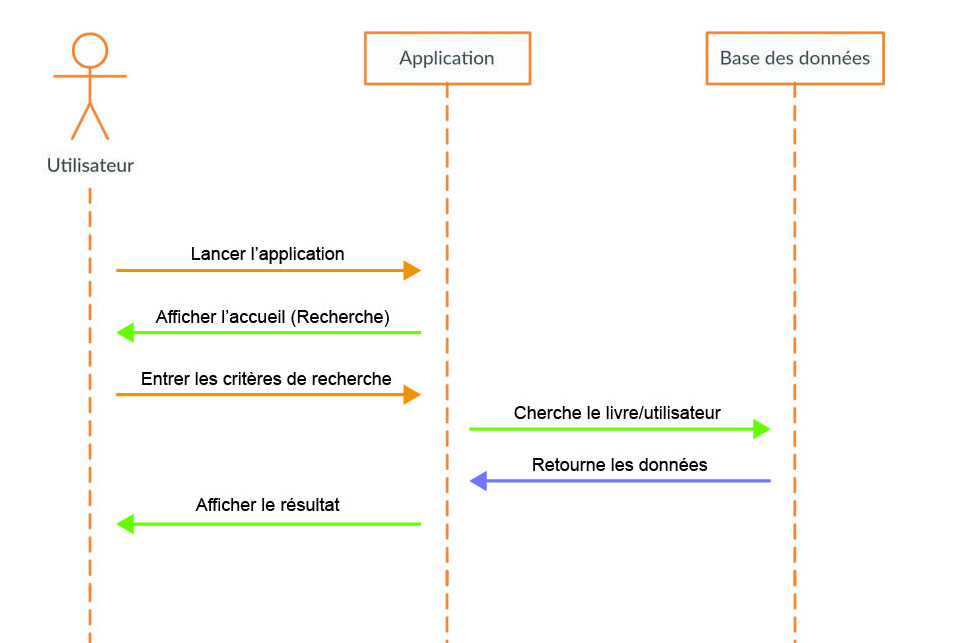
\includegraphics[width=8cm]{Images/chapter3/rechercher_un_livre.jpg}
		\caption{{\footnotesize l'enchaînement des actions pour la recherche d'un  livre particulier}}
	\end{center}
\end{figure}

\begin{figure}[h]
	\begin{center}
		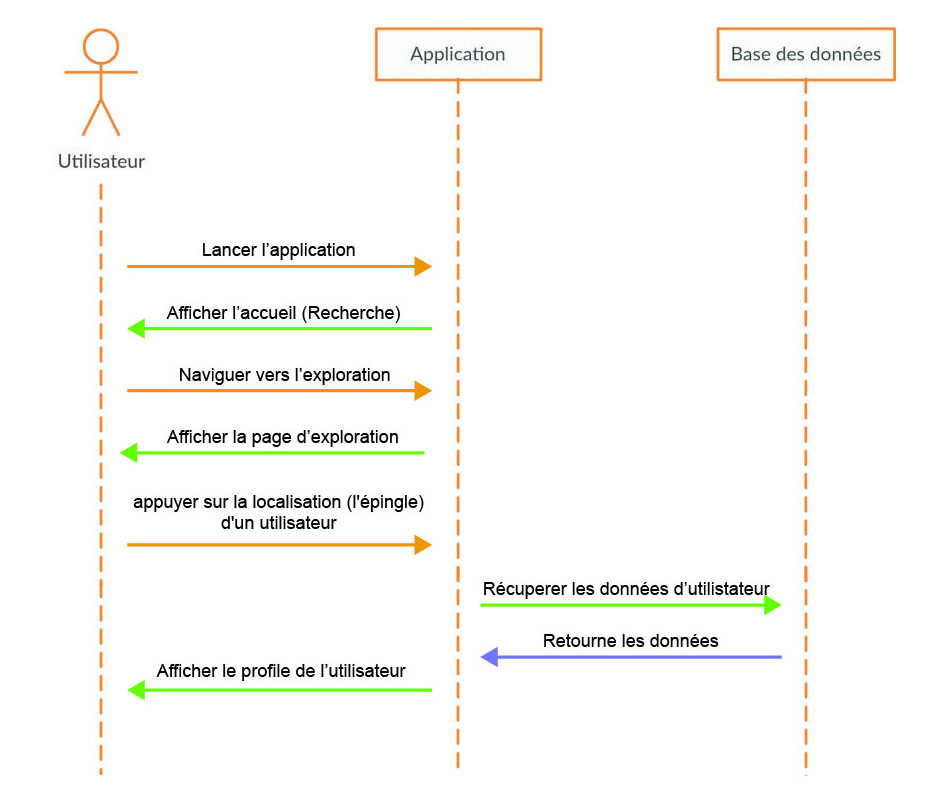
\includegraphics[width=8cm]{Images/chapter3/explorer_les_livres.jpg}
		\caption{{\footnotesize l'exploration des livres/utilisateurs à proximité}}
	\end{center}
\end{figure}

\newpage

\subsubsection{Diagramme de navigation}

\begin{figure}[h]
	\begin{center}
		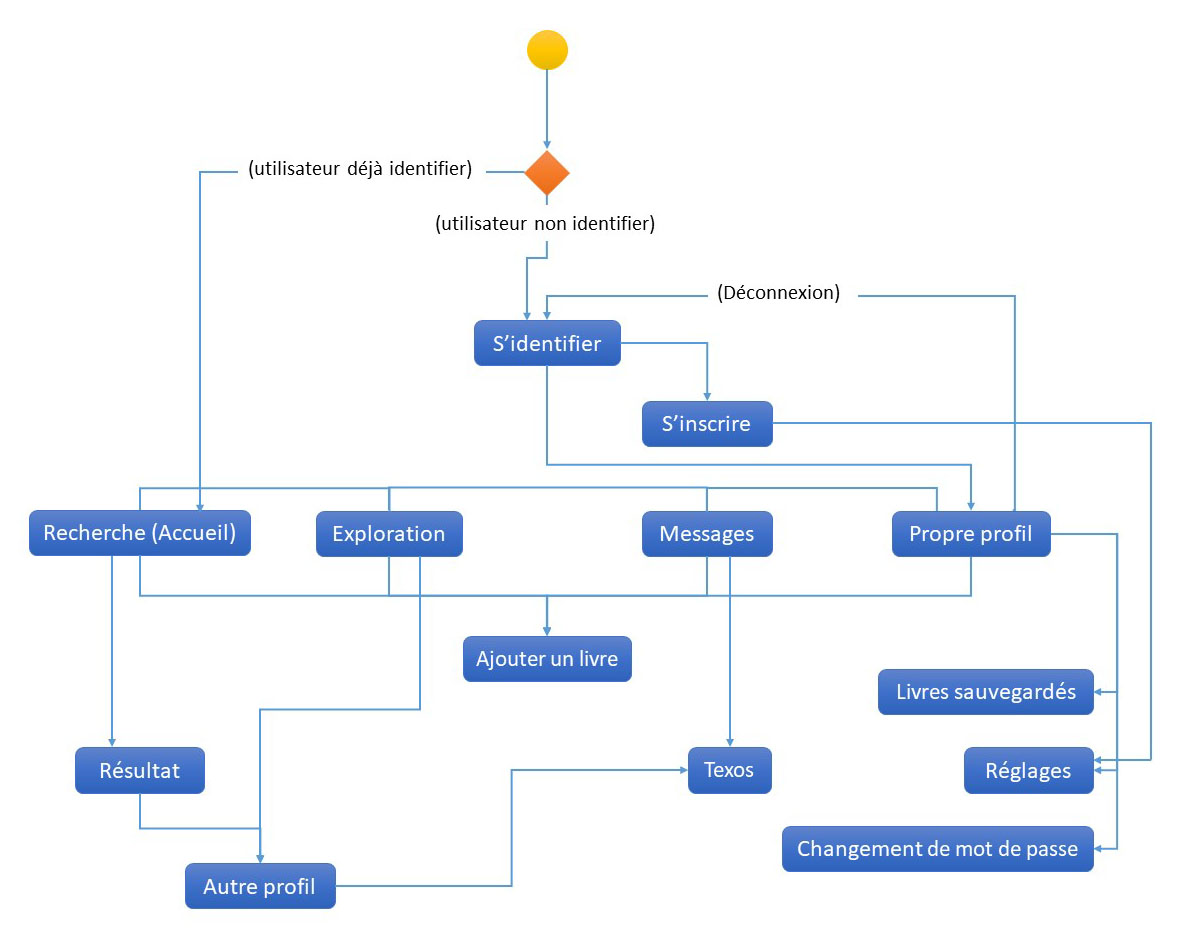
\includegraphics[width=14cm]{Images/chapter3/diagramme_de_navigation.jpg}
		\caption{{\footnotesize l'architecture de navigation}}
	\end{center}
\end{figure}

\subsection{Maquette fonctionnelle (Wireframe)}
Le wireframe ou maquette fonctionnelle est un schéma utilisé lors de la conception d'une interface pour définir les zones et composants qu'elle doit contenir. À partir d'un wireframe peut être réalisée l'interface proprement dite par un graphiste. La démarche de recourir à des wireframes s'inscrit dans une recherche d'ergonomie. Elle est surtout utilisée dans le cadre du développement logiciel et des sites et applications Web. Le wireframe consiste concrètement en un croquis, un collage papier ou un schéma numérique\cite{noauthor_wireframe_nodate}.




\section{Implémentation}

\newpage

\chapter*{Conclusion \& perspective}

\addcontentsline{toc}{chapter}{Conclusion \& perspective}
Le travail présenté dans ce mémoire licence décrit les outils et les étapes, ainsi que la base de connaissances nécessaire à la création d'une application mobile, qui est une plate-forme qui sert à faciliter le processus d'échange de livres entre lecteurs en fonction de leur localisation géographique.\medskip

Tout au long du parcours visant à donner vie à ce projet, et pour le fait que c’était un projet conjoint entre deux étudiants. quelques leçons importantes ont été apprises, Tout d’abord, je crois que maintenant nous réalisons tous les deux vraiment la valeur de publier un document détaillé et très spécifique. À la fin de chaque étape du processus, ainsi que la communication entre les créateurs du projet étant très crucial., et ça sans parler des connaissances techniques et de l'expérience véritablement acquises, de la conception de l'interface utilisateur à l'utilisation efficace de la documentation logicielle en ligne.\medskip

Ce travail n’est pas un projet achevé, et nous n’avions pas l’intention de le rendrait. Nous voulions que ce projet soit une excellente expérience d’apprentissage qui, d’une manière primordiale, devrait remettre en défi notre zone de confort et nos compétences. À des fins particulières, un framework nouvellement créé a été utilisé, et par un langage de programmation qui, avant ce projet, aucun de nous ne le connaissait. Et parce que nous manquions volontairement d'expérience et de connaissances sur la technologie que nous utilisions, nous avons adopté une stratégie qui s'est révélée efficace dans nos circonstances actuelles. Elle consistait à créer d'abord la partie frontale de l'application, indépendamment du \gls{back-end} avec des données factices (\gls{dummy data}), puis travaillez progressivement à remplacer ces fausses données par des données réelles extraites des serveurs.\medskip

Cette première version de l'application peut servir autant qu'un \acrshort{MVP} (Minimum viable product) très utile. En utilisant les outils d'analyse de données fournis par Firebase, nous pouvons facilement étudier le comportement de nos utilisateurs et émettre des hypothèses sur la manière d'optimiser davantage notre expérience utilisateur tout en ajoutant de nouvelles fonctionnalités et en élargissions ce que ce produit peut réaliser. Cependant, avant même d’obtenir les commentaires de nos utilisateurs, nous étions encore en mesure de formuler des hypothèses sur ce qui pouvait être ajouté à l’application et ce qui pouvait être amélioré pour le mieux:

\begin{description}

\item[• Images réelles:] pour le moment, et afin de garder une interface utilisateur propre, nous avons choisi de ne pas donner la liberté d'ajouter de nombreuses images d'un livre. Nous avons insisté pour que les utilisateurs utilisent des couvertures numérisées plutôt que photographiées. Je pense que cette limitation que nous avons dû imposer aux utilisateurs ne durera pas longtemps, car l'expérience utilisateur sera de plus en plus personnalisable.

\item[• Suivi des transactions:] nous supposons que la mise en place d'un mécanisme de suivi des transactions peut être très bénéfique pour les utilisateurs, en particulier ceux qui prêtent plusieurs livres et aiment savoir où se trouvent leurs livres et quand ils ont été prêtés.

\item[• Découverte de livres:] pour les aventuriers qui ne savent pas exactement ce qu’ils recherchent, nous pouvons ajouter différentes méthodes pour trouver des livres, par exemple: présenter divers livres appartenant à des personnes géographiquement proches et les présenter un par un, où l'utilisateur voit les détails ou ignore chaque option.

\item[• Suggestion de livres:] compte tenu de la quantité de données que nous pouvons obtenir de la liste de livres de chaque utilisateur et des requêtes de recherche qu’il entre, nous pouvons implémenter une fonction de suggestion sous forme de notification push concernant les livres qu’un utilisateur pourrait trouver intéressants.

\item[• Une meilleure architecture logicielle:] au fur et à mesure que l'application évoluera, le maintien et la modification des fonctionnalités de l'application s'avéreront fastidieux. La prochaine décision rationnelle consistera donc à mieux structurer l'application de manière à permettre un processus de dimensionnement en douceur.

\end{description}



\bibliographystyle{plain}
\bibliography{bibli}


\newpage

\thispagestyle{empty}

\vspace*{2cm}

\begin{center}
\textbf{Résumé}
\end{center}

Les livres ont toujours été le principal vecteur de connaissances tout au long de l'histoire, et l'une des pratiques les plus gratifiantes connues de l'humanité, heureusement, de nos jours encore, une grande partie de la population considère la lecture comme un mode de vie et le livre comme le meilleur compagnon qu'une personne puisse espérer avoir. Cependant, dans le monde actuel et plus particulièrement dans notre pays, l'Algérie, ce mode de vie est devenu de plus en plus difficile à maintenir, pour des raisons aussi diverses que le coût d'achat de certains livres, la difficulté d'en trouver d'autres et les difficultés rencontrées pour se connecter à d'autres lecteurs qui partagent les mêmes intérêts et amour pour la lecture.\medskip

Par conséquent, afin de résoudre ces problèmes, nous nous sommes tournés vers la technologie, en exploitant le pouvoir offert par les smartphones qui envahissent tous les poches et l’énorme popularité des réseaux sociaux, nous avons décidé de concevoir et de mettre en œuvre une application mobile.\medskip

Cette application mobile permet aux utilisateurs de définir un profil avec leur localisation géographique et de répertorier tous les livres qu'ils possèdent et qu’ils sont prêts à les prêtés, cédés, vendus ou échangés contre un autre livre avec un autre utilisateur. Cela leur permet également de parcourir le profil d'autres utilisateurs. Et leurs listes de livres dans l’espoir de trouver un livre qui les intéresse ou même un ami avec qui partager la passion de la lecture.\medskip

Nous avons pu ouvrir la voie en créant une conception détaillée et, plus tard, en développant les principales fonctionnalités en tenant compte des améliorations potentielles.

\end{document}
